%!TEX root = /Users/ego/Boulot/Alterqcm/doc/doc_aq-main.tex    

\section{Exemples complémentaires} 
\subsection{Les symbolistes :  usage de la macro \tkzcname{includegraphics}}  
\Imacro{includegraphics}

\begin{alterqcm}[lq=8cm,numprop=true,sep]
\AQquestion[pq=2 cm]{Parmi les trois tableaux ci-contre, quel est celui peint par \textbf{Gustave Moreau}\vfill}%
{{%
\hfil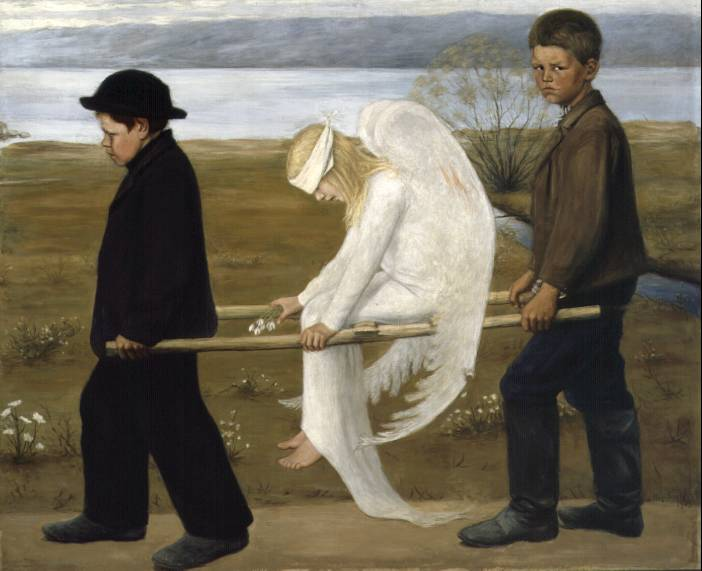
\includegraphics[scale=.20]{The_Wounded_Angel_-_Hugo_Simberg.jpg}\hfil
},{%
\hfil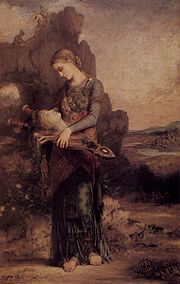
\includegraphics[scale=.4]{180px-Gustave_Moreau_007.jpg}\hfil
},{%
\hfil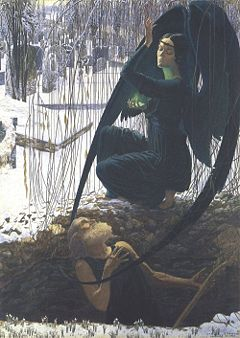
\includegraphics[scale=.4]{240px-Mort_du_fossoyeur.jpg}\hfil}}%
 \AQquestion[pq=1 cm]{Le tableau suivant a été peint par lequel de ces trois peintres ?\\
\hfil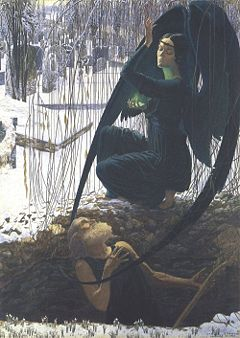
\includegraphics[height=3in]{240px-Mort_du_fossoyeur.jpg}\hfil}%
{{Gustav Klimt},{Carlos Schwabe},{Odilon Redon}}
\end{alterqcm} 

\begin{tkzltxexample}[small]
 \begin{alterqcm}[lq=8cm,numprop=true,sep]
 \AQquestion[pq=2 cm]{Parmi les trois tableaux, quel est celui peint par \textbf{Gustave Moreau}\vfill}%
 {{%
 \hfil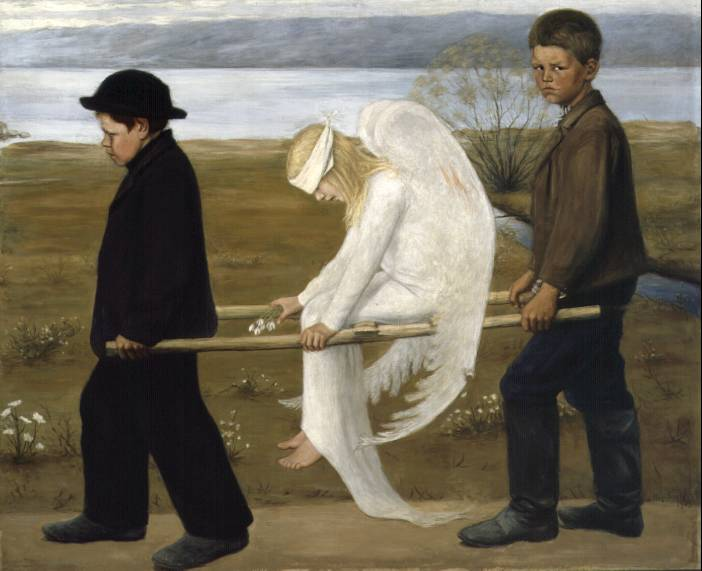
\includegraphics[scale=.25]{The_Wounded_Angel_-_Hugo_Simberg.jpg}\hfil
 },{%
 \hfil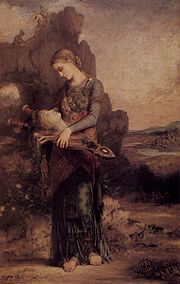
\includegraphics[scale=.5]{180px-Gustave_Moreau_007.jpg}\hfil
 },{%
 \hfil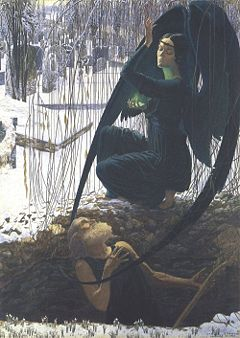
\includegraphics[scale=.4]{240px-Mort_du_fossoyeur.jpg}\hfil}}
  \AQquestion[pq=1 cm]{Le tableaux suivant, a été peint par lequel de ces trois peintres ?\\
 \hfil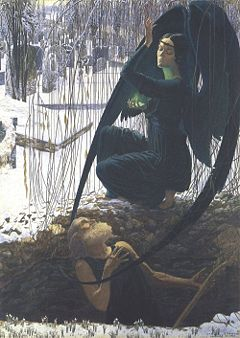
\includegraphics[height=3in]{240px-Mort_du_fossoyeur.jpg}\hfil}%
 {{Gustav Klimt},{Carlos Schwabe},{Odilon Redon}}
 \end{alterqcm} 
\end{tkzltxexample}

\subsection{Emploi d'un environnement \tkzname{tikzpicture} dans une question} 
\Ienv{tikzpicture}

\medskip

\begin{alterqcm}[lq=120mm,pre=true,pq=3mm]
 \AQmessage{\begin{minipage}{15cm}
\vspace*{6pt}   
Les trois arbres donnés ci-dessous représentent des situations probabilistes. %
  Les nombres indiqués sur les différentes flèches sont des  probabilités, et,%
    en deuxième niveau,  des probabilités conditionnelles. Ainsi pour l'arbre donné %
      dans la question 1 : $0,35 = P(A)$ et $0,1 =  P_{\text{A}}(E)$.
\vspace*{6pt}    
\end{minipage}  
}
\AQquestion{La probabilité de l'événement E est égale à : \\
\begin{tikzpicture}[yscale=1.2] 
[parent anchor=east,child anchor=west,grow=east]
\tikzstyle{every node}=[text=Maroon,fill=fondpaille,font=\small]
\tikzstyle{every child}=[level distance=25mm]
\tikzstyle{edge from parent}=[draw,->,thin] 
\tikzstyle{level 2}=[sibling distance=12mm]
\node {}
[grow=right]   
child {node {B}
      child { node {F}
        edge from parent node {$0,5$}}
      child { node {E}
        edge from parent node {$0,5$}
            }
         edge from parent node {$0,65$}
       }
child {node {A}
        child { node {F}
          edge from parentnode {$0,9$}}
        child { node {E}
          edge from parent node {$0,1$}}
      edge from parent node {$0,35$}
      };
\end{tikzpicture}}
{{$0,5$},%
{$0,1$},%
{$0,6$},%
{$0,36$}}
\end{alterqcm} 

\begin{tkzltxexample}[small]
 \begin{alterqcm}[lq=120mm,pre=true,pq=3mm]
  \AQmessage{Les trois arbres donnés ci-dessous représentent des situations probabilistes.
   Les nombres indiqués sur les différentes flèches sont des  probabilités, et,
   en deuxième niveau,  des probabilités conditionnelles. Ainsi pour l'arbre donné 
   dans la question 1 : $0,35 = P(A)$ et $0,1 =  P_{\text{A}}(E)$.}
 \AQquestion{La probabilité de l'événement E est égale à : \\
 \begin{tikzpicture} 
 ...
 \end{tikzpicture}}
 {{$0,5$},%
 {$0,1$},%
 {$0,6$},%
 {$0,36$}}
 \end{alterqcm} 
\end{tkzltxexample}

\subsection{Emploi d'un environnement \tkzname{array} dans les propositions} 
\Ienv{array}

Il est possible d'utiliser des tableaux ainsi que d'autres structures dans le code de la question ou encore des propositions. Voici un exemple :

\medskip


\begin{tkzexample}[vbox]
\begin{alterqcm}[lq=88mm,symb=$\Box$]
\AQquestion{Le couple $(1~;~-1)$ est solution de }
{%
{$ \left\lbrace
\begin{array}{ll}
 0,75a + 0,5b &= 0,25 \\
 0,25a + 0,5b &=-0,25
\end{array}\right.$},
{$ \left\{
\begin{array}{ll}
 a &=  0,75a +0,5b \\
 b &=  0,25a +0,5b
\end{array}\right.$},
{$ \left\lbrace
\begin{array}{ll}
 0,75a - 0,5b &= 0,25 \\
 0,5a + 0,25b &=-0,25
\end{array}\right.$}
}
\end{alterqcm}\end{tkzexample}  

\subsection{Emploi d'un environnement \tkzname{tikzpicture} dans une question} 
\Ienv{tikzpicture}

\begin{tkzexample}[vbox]
\begin{alterqcm}[lq=8cm,numprop=true,sep]
\AQquestion{Parmi les figures ci-contre, indiquer celle qui est un losange :}
{{\hspace{1cm}  \begin{minipage}{5cm} 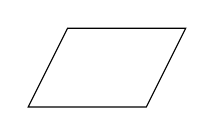
\begin{tikzpicture} 
  \draw (0,0)--(1.5,0)--(2,1)--(.5,1)--cycle; 
\end{tikzpicture} \end{minipage}},
{\hspace{1cm}  \begin{minipage}{5cm} 
\begin{tikzpicture}
   \draw[rotate=30] (0,0) rectangle (1.5,1); \end{tikzpicture} \end{minipage}},
{\hspace{1cm}  \begin{minipage}{5cm} 
\begin{tikzpicture}
   \draw (0,0) rectangle (1,1); \end{tikzpicture} \end{minipage} }}
\end{alterqcm} 
\end{tkzexample}

\subsection{Emploi de code \tkzname{verbatim} dans les questions et les propositions} 
\Ienv{verbatim}

Voici un exemple de Pascal Bertolino. Il est préférable d'utiliser comme Pascal l'a fait la macro \tkzcname{texttt}, autrement d'éviter l'usage du mode 
|verbatim|. Nous verrons à la page suivante comment procéder si ce mode est réellement nécessaire.

\begin{alterqcm}[lq=80mm,title=false,long] 

%--------------------------------------------------------------
\AQquestion{Quel était le langage précurseur du langage C ?}
{{le Fortran},
 {le langage B},
 {le Basic}}

%--------------------------------------------------------------
\verbdef\argprop|int a = 3 ^ 4 ;|
\AQquestion{\argprop}
{{élève 3 à la puissance 4},
 {fait un OU exclusif entre 3 et 4},
 {n'est pas une instruction C}}

%--------------------------------------------------------------
\AQquestion{Quelle est la bonne syntaxe pour décaler de 8 bits à gauche l'entier \texttt{a} ?}
{{\texttt{b = lshift(a, 8) ;}},
 {\texttt{b = 8 << a ;}},
 {\texttt{b = a << 8 ;}}}
%--------------------------------------------------------------
\verbdef\argprop|{ printf ("bonjour") ; return 0 ; \}|
\AQquestion{Le programme complet :	\\
\texttt{int main() \\
~~\argprop}}
{{affiche \texttt{bonjour}},
 {donne une erreur à la compilation},
 {donne une erreur à l'exécution}}
%--------------------------------------------------------------
\verbdef\arg|float tab[10]|
\verbdef\propa|*tab|\global\let\propa\propa
\verbdef\propb|&tab|\global\let\propb\propb
\verbdef\propc|tab|\global\let\propc\propc
\AQquestion{Soit la déclaration \arg ; \\Le premier réel du tableau  est \ldots}
{{\propa},
 {\propb},
 {\propc}}

%--------------------------------------------------------------
\AQquestion{La ligne \texttt{printf("\%c", argv[2][0]) ;} du \texttt{main} de  \texttt{monProg} exécuté ainsi : 
\texttt{monProg parametre }}
{{affiche \texttt{p}},
 {n'affiche rien},
 {peut provoquer un plantage}}
%--------------------------------------------------------------
\AQquestion{Quelle est la taille en mémoire d'un \texttt{long int} ?}
{{4 octets},
 {8 octets},
 {ça dépend \ldots}}
%--------------------------------------------------------------
\AQquestion{Suite à la déclaration \texttt{int * i} ;}
{{\texttt{*i} est une adresse},
 {\texttt{*i} est un entier},
 {\texttt{*i} est un pointeur}}
%--------------------------------------------------------------
\AQquestion{Un des choix suivants n'est pas une bibliothèque standard du C}
{{\texttt{stdlib}},
 {\texttt{stdin}},
 {\texttt{math}}}

\end{alterqcm}

\medskip
Voyons le code source

le plus simple est souvent d'utiliser la commande \tkzcname{texttt}

\medskip
\begin{tkzexample}[code only]
 \AQquestion{Suite à la déclaration \texttt{int * i} ;}
 {{\texttt{*i} est une adresse},
 {\texttt{*i} est un entier},
 {\texttt{*i} est un pointeur}}
\end{tkzexample}

\medskip
\begin{tkzexample}[code only]
\AQquestion{La ligne \texttt{printf("\%c", argv[2][0]) ;}
 du \texttt{main} de  \texttt{monProg} exécuté ainsi : 
\texttt{monProg parametre }}
{{affiche \texttt{p}},
 {n'affiche rien},
 {peut provoquer un plantage}}
\end{tkzexample}

\medskip
Sinon on peut charger le package \tkzname{verbdef} :
\NamePack{verbdef}

\medskip
\tkzcname{usepackage\{verbdef\}}

\medskip
\begin{tkzexample}[code only]
 \verbdef\argprop|int a = 3 ^ 4 ;|
 \AQquestion{\argprop}
 {{élève 3 à la puissance 4},
  {fait un OU exclusif entre 3 et 4},
  {n'est pas une instruction C}}
\end{tkzexample}

\medskip
Il est possible que plusieurs variables soient nécessaires :

\medskip

\begin{tkzexample}[code only]
 \verbdef\arg|float tab[10]|
 \verbdef\propa|*tab|\global\let\propa\propa
 \verbdef\propb|&tab|\global\let\propb\propb
 \verbdef\propc|tab|\global\let\propc\propc
 \AQquestion{Soit la déclaration \arg ; \\
 Le premier réel du tableau  est \ldots}
 {{\propa},
  {\propb},
  {\propc}}
\end{tkzexample}



\endinput